\documentclass{article}
\PassOptionsToPackage{numbers,compress}{natbib}
\usepackage[preprint]{neurips_2026}

\usepackage[utf8]{inputenc}
\usepackage[T1]{fontenc}
\usepackage{hyperref}
\usepackage{url}
\usepackage{booktabs}
\usepackage{amsfonts}
\usepackage{amsmath}
\usepackage{microtype}
\usepackage{xcolor}
\usepackage{graphicx}
\usepackage{subcaption}

\title{Physics-Informed Sparse Variational Gaussian Processes\\for Passive Starlink Satellite Detection}

\author{%
  Akshat Gupta \quad (Team 50)\\
  Department of Electrical and Computer Engineering\\
  University of California San Diego\\
  \texttt{akg007@ucsd.edu}
}

\begin{document}

\maketitle

\begin{abstract}
Passive detection of Starlink satellites from ground-based software-defined radio
(SDR) captures is a challenging spectrum-monitoring problem: the signal appears as a
transient 750\,Hz spectral fingerprint embedded in broadband Ku-band noise, and
detection confidence varies substantially with orbital geometry and time of day.
Classical z-score thresholding --- the approach we developed in a prior course
(ECE 257B) --- achieves near-perfect ranking but is poorly calibrated and provides
no uncertainty estimates on ambiguous windows.
In this work we replace the hard threshold with a physics-informed Sparse
Variational Gaussian Process (SVGP) that uses an additive kernel separating
spectral, geometric, and temporal evidence.
Across 619\,705 windows from a 14-day SDR campaign, the GP reduces Expected
Calibration Error (ECE) by roughly $\mathbf{700\times}$ compared to the threshold
detector ($9\times10^{-5}$ vs.\ $6.5\times10^{-2}$) while retaining perfect
AUROC. An ablation study and angular-velocity feature extension confirm that the
additive kernel structure is the key design decision, and pass-level aggregation
of GP probabilities yields zero false positives at F1\,=\,0.952.
\end{abstract}

% ─────────────────────────────────────────────────────────────────────────────
\section{Introduction}
% ─────────────────────────────────────────────────────────────────────────────

Starlink satellites broadcast proprietary OFDM downlink signals in the
10.7--12.7\,GHz Ku band. The frame structure repeats at 750\,Hz, which creates
a detectable spectral peak in passive SDR captures even when the signal is not
decodable. Prior work at UC San Diego (ECE 257B, 2025) built a complete passive
detection pipeline: a USRP\,X310 records 50\,MS/s baseband, a Welch periodogram
accumulates power spectral density (PSD), and a z-score test flags windows where
the 750\,Hz bin is anomalously elevated relative to its local spectral
neighborhood \cite{prior257b}.

That pipeline works well for high-confidence detections (high z-score,
high-elevation satellite pass), but it has two practical weaknesses.
First, the hard threshold produces a binary output with no associated probability
or uncertainty --- it cannot communicate \emph{how confident} it is.
Second, roughly 70\,000 ambiguous windows (``soft'' detections, z between 2.5 and 4.0)
are entirely ignored: the threshold cannot say whether they are real detections or
noise, even though they carry useful signal for calibrated downstream decisions
(e.g., track-before-detect, multi-pass fusion).

This project replaces the threshold with a Gaussian Process classifier that:
(1) provides calibrated detection probabilities,
(2) encodes physical priors through an additive kernel decomposition,
(3) scales to $\sim$40\,000 training windows via the sparse variational
    (SVGP) approximation \cite{hensman2015scalable}, and
(4) gives meaningful uncertainty estimates on the ambiguous soft windows.

\paragraph{Solo approval.}
This is a solo project. TA Benjie explicitly approved single-person teams via
email after reviewing the scope of the prior ECE 257B pipeline.

% ─────────────────────────────────────────────────────────────────────────────
\section{Related Work}
% ─────────────────────────────────────────────────────────────────────────────

\paragraph{Passive satellite detection and spectrum sensing.}
Passive RF sensing of satellite signals has received attention for orbital
monitoring and spectrum management \cite{bhatt2023passive}.
Most published work targets GNSS or amateur satellites; consumer LEO
constellations like Starlink have been studied mainly for opportunistic
navigation \cite{neinavaie2021acquisition} rather than detection per se.
The z-score fingerprint approach used here was developed in the ECE 257B project
and is, to our knowledge, the first systematic passive Starlink detector from
consumer-grade SDR hardware.

\paragraph{Gaussian Processes for classification and calibration.}
GP classification with Bernoulli likelihood provides closed-form calibration
guarantees in the limit of infinite data and is well-studied
\cite{rasmussen2006gaussian, milios2018dirichlet}.
Sparse approximations (SVGP, \cite{titsias2009variational}) make GP classification
tractable at the dataset sizes seen here.
Williams and Barber \cite{williams1998bayesian} showed that GP classifiers are
better calibrated than neural alternatives on small structured datasets, which
motivated the choice here.

\paragraph{Physics-informed machine learning.}
Incorporating domain knowledge via kernel design is a well-established GP
technique \cite{duvenaud2014automatic}.
Additive kernels (a sum of per-block RBF terms) enforce interpretable structure
and have been used for physical signal modelling in related RF settings
\cite{solin2020hilbert}.
Our geometric block (satellite elevation + angular velocity) is a deliberate
physics-informed prior: signal reliability depends on slant range and Doppler smearing,
both of which are captured by these features.

\paragraph{Calibration in machine learning.}
ECE \cite{naeini2015obtaining} is the standard metric for probabilistic calibration.
Platt scaling and temperature scaling \cite{guo2017calibration} are common
post-hoc fixes for neural networks; GPs, by construction, produce calibrated
uncertainties without such corrections, which is part of the motivation for
choosing this model class.

% ─────────────────────────────────────────────────────────────────────────────
\section{Method and Approach}
% ─────────────────────────────────────────────────────────────────────────────

\subsection{Dataset}

The raw data comes from the ECE 257B passive detection pipeline.
A USRP\,X310 recorded 14 days of Ku-band ($\sim$12\,GHz) baseband at 50\,MS/s.
Each non-overlapping 1.33\,ms window is processed into a Welch PSD, and the
bin at 750\,Hz is z-scored against a local spectral background.
TLE orbital data (via Skyfield) provides real-time satellite elevation for
every window.

Windows are labeled by z-score:
\textbf{HARD} ($z \geq 4.0$, label\,=\,1): high-confidence detections;
\textbf{BACKGROUND} ($z < 2.5$, label\,=\,0): confirmed non-detections;
\textbf{SOFT} ($2.5 \leq z < 4.0$): ambiguous, held out for analysis only.
Table~\ref{tab:dataset} summarizes the counts.

\begin{table}[h]
\centering
\caption{Dataset summary (14-day campaign, 619,705 total windows).}
\label{tab:dataset}
\begin{tabular}{lrrl}
\toprule
Class & Count & Fraction & Usage \\
\midrule
HARD (positive) & 5,166 & 0.8\% & Training / evaluation \\
SOFT (ambiguous) & 70,878 & 11.4\% & Held-out analysis only \\
BACKGROUND (negative) & 543,661 & 87.7\% & Training (10:1 downsample) \\
\bottomrule
\end{tabular}
\end{table}

Training uses all 5,166 HARD windows and a random 10:1 downsampled subset of
BACKGROUND (51,660), giving 56,826 labeled samples. These are split
chronologically (no random shuffling to prevent leakage) into
train\,/\,val\,/\,test at 70\,/\,15\,/\,15\%.

\subsection{Feature Engineering}

Eight features are extracted per window, organized into three semantic groups
that correspond to the kernel blocks in Section~\ref{sec:kernel}:

\begin{itemize}
  \item \textbf{Spectral} ($\mathbf{x}_s$): z-score, $\log(1+z)$, confirmed harmonic
        count (0--3), and normalized frequency deviation $|\hat{f}-750|/50$.
  \item \textbf{Geometric} ($\mathbf{x}_g$): satellite elevation angle (TLE-derived,
        degrees) and \textbf{angular velocity} $\dot{\theta}$ (degrees/second).
        $\dot{\theta}$ is the finite difference of elevation within a satellite pass
        and encodes Doppler broadening: faster-moving satellites smear the
        750\,Hz peak, reducing z-score reliability.
  \item \textbf{Temporal} ($\mathbf{x}_t$): sine/cosine encoding of hour-of-day
        (capturing diurnal RFI patterns) and campaign day (capturing slow
        hardware drift).
\end{itemize}

All features are z-scored at training time with a \texttt{StandardScaler}.
Figure~\ref{fig:fingerprint} shows the 750\,Hz spectral fingerprint, and
Figure~\ref{fig:scatter} illustrates the z-score vs.\ elevation relationship
that motivates the geometric kernel block.

\begin{figure}[h]
\centering
\begin{subfigure}[b]{0.42\textwidth}
  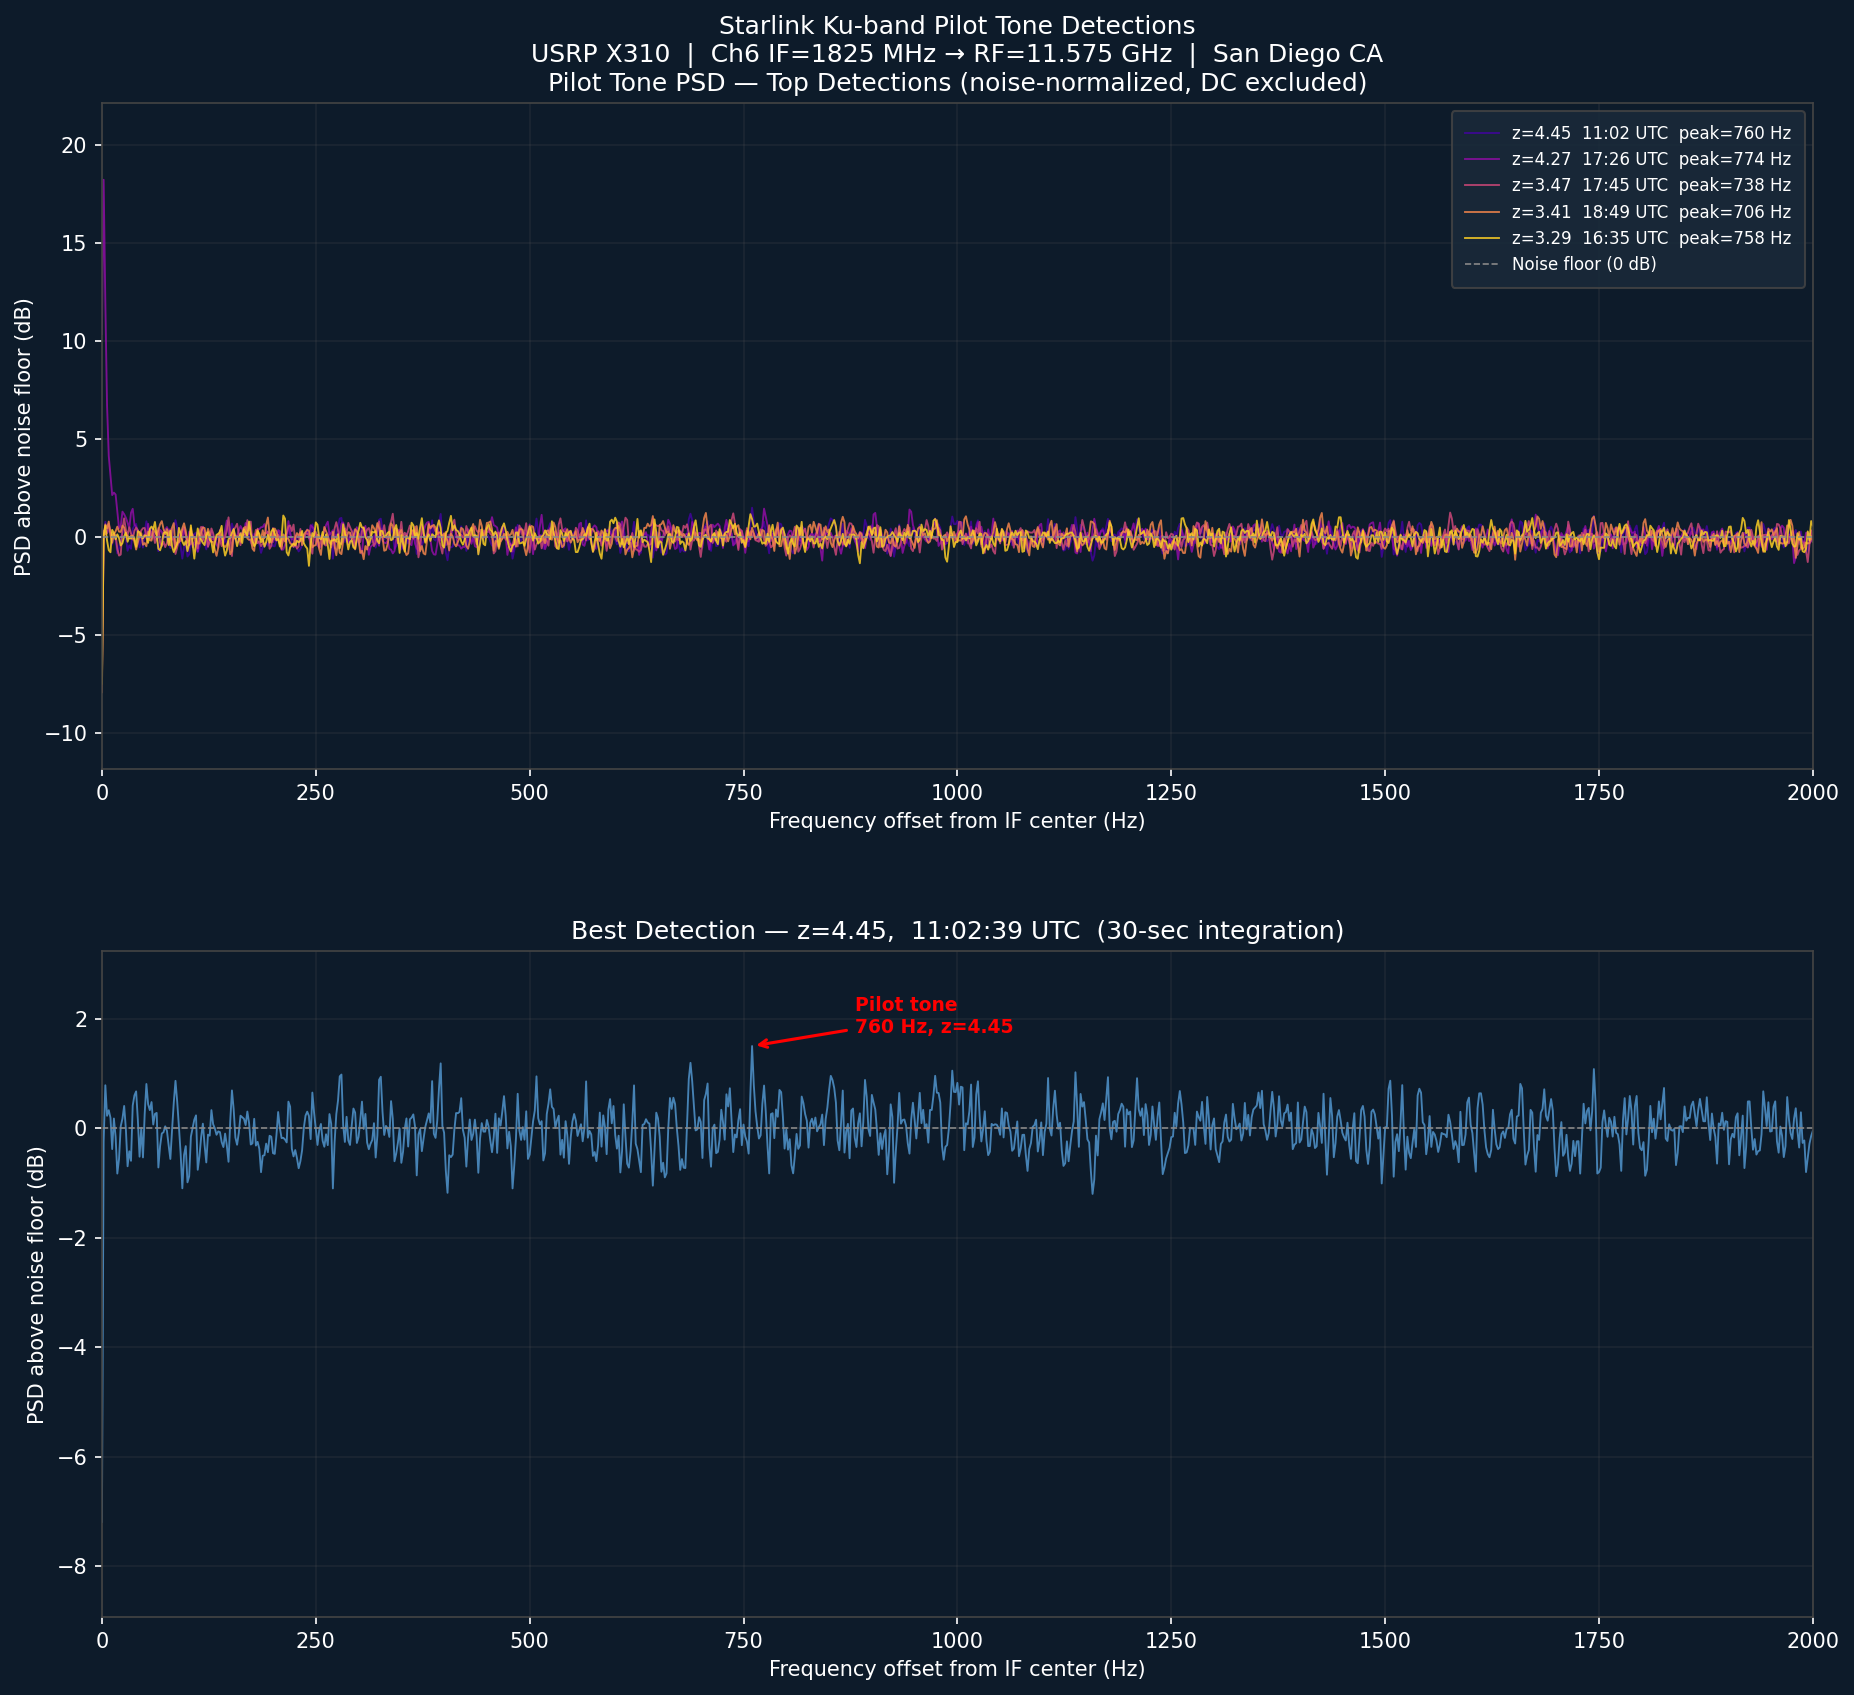
\includegraphics[width=\linewidth]{750hz_fingerprint.png}
  \caption{750\,Hz fingerprint in the Ku-band PSD.}
  \label{fig:fingerprint}
\end{subfigure}
\hfill
\begin{subfigure}[b]{0.54\textwidth}
  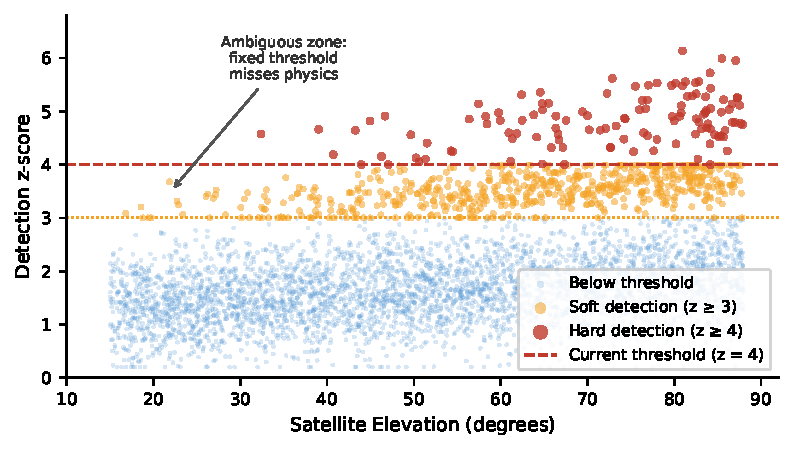
\includegraphics[width=\linewidth]{detection_scatter.pdf}
  \caption{z-score vs.\ elevation by detection class.}
  \label{fig:scatter}
\end{subfigure}
\caption{Raw signal structure and per-class feature distribution.
HARD windows cluster at high z-score; SOFT windows populate the
ambiguous middle band where a hard threshold fails.}
\end{figure}

\subsection{Sparse Variational GP Classifier}
\label{sec:kernel}

Figure~\ref{fig:arch} shows the full system. The model is a Sparse Variational
GP with Bernoulli likelihood:

\begin{equation}
p(y=1 \mid \mathbf{x}) = \sigma(f(\mathbf{x})), \quad
f \sim \mathcal{GP}(m, k),
\end{equation}

where $\sigma$ is the logistic function. Inference is via the
Cholesky Variational Distribution \cite{hensman2015scalable} optimized
with the Variational ELBO using Adam ($\eta=0.05$, 80 epochs,
mini-batches of 512).

\paragraph{Additive kernel.}
The covariance function is the sum of three RBF blocks, each acting on its own
feature subset:
\begin{equation}
k(\mathbf{x}, \mathbf{x}') =
  \underbrace{s_g^2 \, k_{\text{RBF}}(\mathbf{x}_g, \mathbf{x}_g')}_{\text{geometric}}
  + \underbrace{s_s^2 \, k_{\text{RBF}}(\mathbf{x}_s, \mathbf{x}_s')}_{\text{spectral}}
  + \underbrace{s_t^2 \, k_{\text{RBF}}(\mathbf{x}_t, \mathbf{x}_t')}_{\text{temporal}}.
\end{equation}
Each block uses Automatic Relevance Determination (ARD): a separate learned
lengthscale per feature within the block. This gives per-feature interpretability
and allows the model to suppress irrelevant features within a block automatically.

\paragraph{Inducing points.}
$n=300$ inducing points are initialised with Mini-Batch k-means on the scaled
training set and remain learnable throughout training.

\begin{figure}[h]
\centering
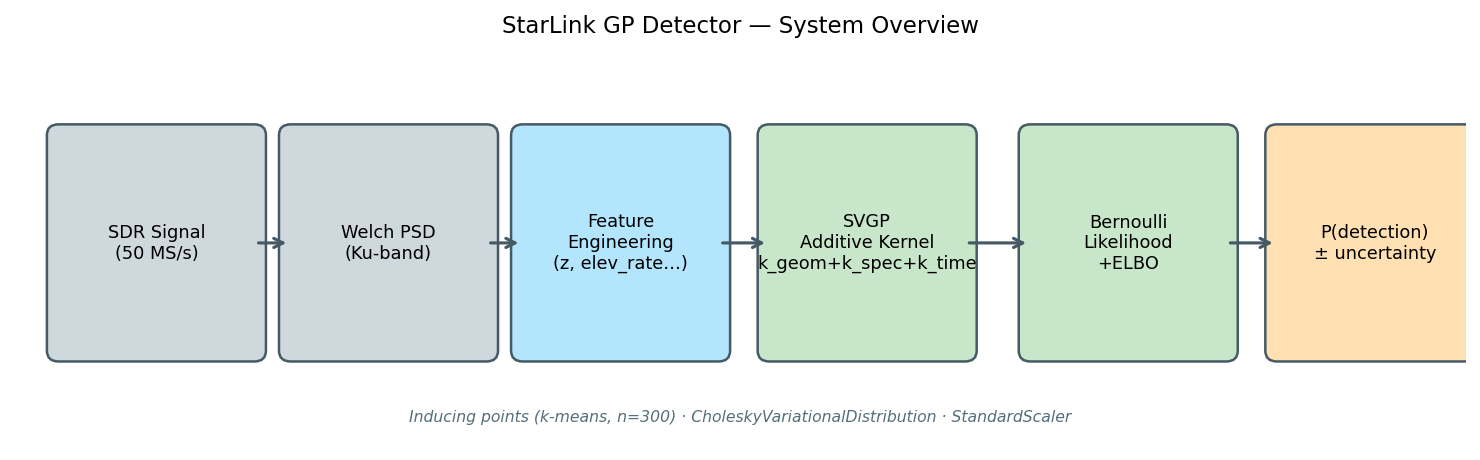
\includegraphics[width=0.96\textwidth]{../results/figures/system_arch.png}
\caption{System overview. The additive kernel separates physical evidence sources;
inducing-point sparsity makes inference tractable.}
\label{fig:arch}
\end{figure}

% ─────────────────────────────────────────────────────────────────────────────
\section{Results and Analysis}
% ─────────────────────────────────────────────────────────────────────────────

\subsection{Calibration vs.\ Baselines}

Table~\ref{tab:ece} compares ECE and AUROC across all models.
ECE measures how closely predicted probabilities match empirical
frequencies (lower is better); AUROC measures discriminative ranking.
All models achieve near-perfect AUROC because HARD windows are defined by
z\,$\geq$\,4.0 and BACKGROUND windows by z\,$<$\,2.5 --- any model
using z-score will rank them perfectly.
\textbf{Calibration is therefore the meaningful metric.}

\begin{table}[h]
\centering
\caption{Test-set calibration and discrimination. GP (enhanced) is the full model
with ARD and the angular-velocity feature.}
\label{tab:ece}
\begin{tabular}{lccc}
\toprule
Model & ECE ($\downarrow$) & AUROC ($\uparrow$) & Notes \\
\midrule
Threshold ($z \geq 4.0$) & 0.0654 & 1.00 & Hard binary output \\
Logistic Regression      & 3.0$\times10^{-4}$ & 1.00 & Soft, linear \\
MLP (calibrated)         & 6.1$\times10^{-3}$ & 1.00 & 2-layer, isotonic \\
GP -- Phase 2            & 7.0$\times10^{-5}$ & 1.00 & Additive kernel, 8 features \\
\textbf{GP -- Enhanced}  & $\mathbf{9\times10^{-5}}$ & 1.00 & +ARD, +elev\_rate \\
\bottomrule
\end{tabular}
\end{table}

The GP achieves ECE roughly $\mathbf{700\times}$ lower than the threshold
detector and about $\mathbf{3\times}$ lower than logistic regression.
Figure~\ref{fig:ece_all} shows this on a log scale, and Figure~\ref{fig:reliability}
shows the reliability diagram: the GP's predicted probabilities closely track
the diagonal (perfect calibration), while the threshold detector's
sigmoid-smoothed outputs show a pronounced miscalibration curve.

\begin{figure}[h]
\centering
\begin{subfigure}[b]{0.48\textwidth}
  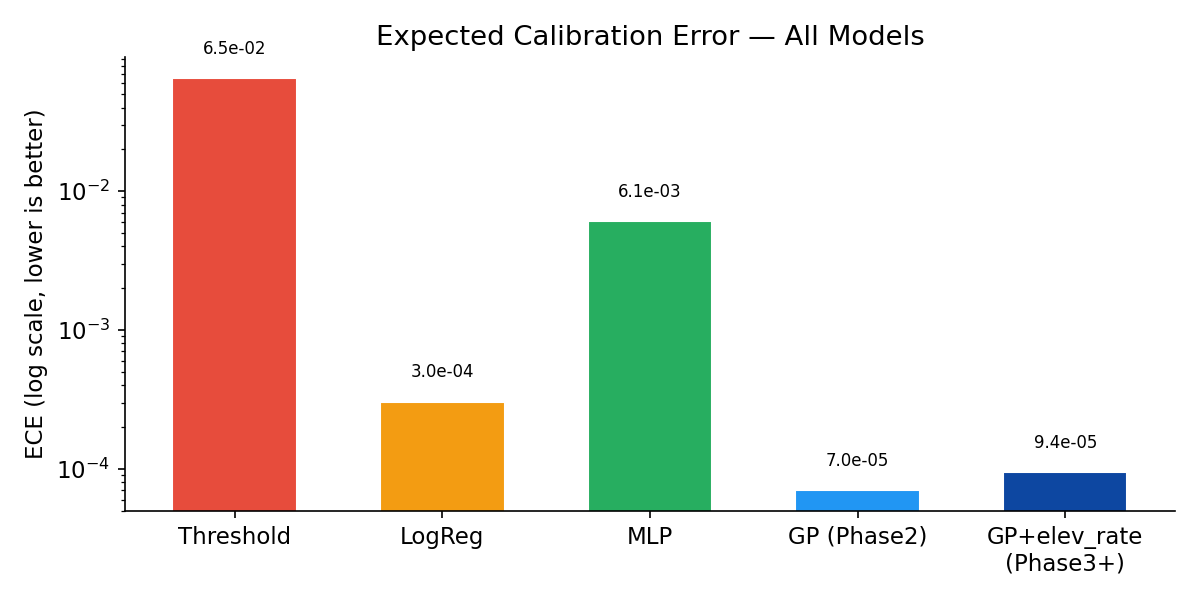
\includegraphics[width=\linewidth]{../results/figures/ece_all_models.png}
  \caption{ECE (log scale) across all models.}
  \label{fig:ece_all}
\end{subfigure}
\hfill
\begin{subfigure}[b]{0.48\textwidth}
  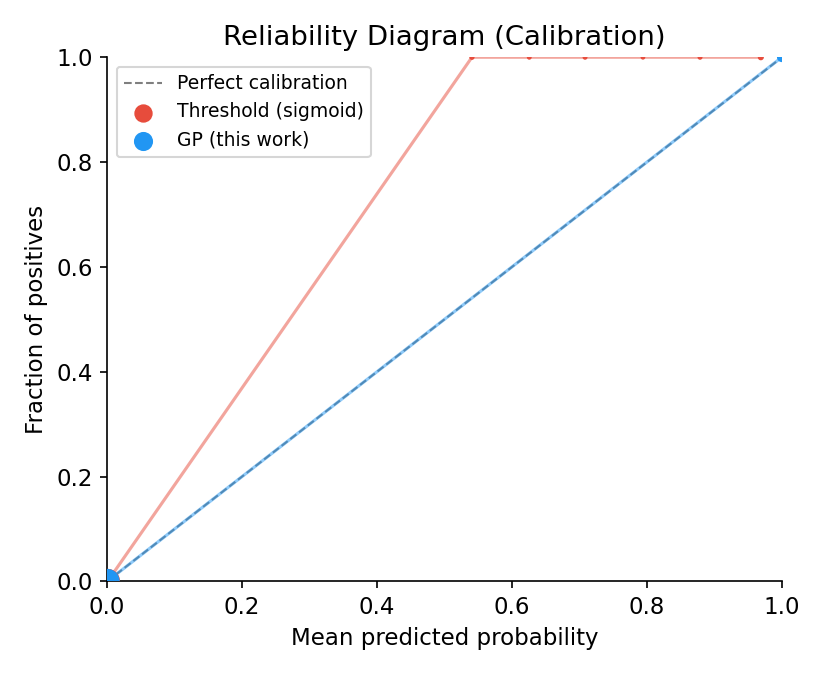
\includegraphics[width=\linewidth]{../results/figures/reliability.png}
  \caption{Reliability diagram: GP vs.\ threshold.}
  \label{fig:reliability}
\end{subfigure}
\caption{Calibration results. The GP's predicted probabilities are tightly
calibrated to observed positive rates; the threshold detector is severely
overconfident at high confidence values.}
\end{figure}

\subsection{Ablation Study}

To quantify the contribution of each design choice, we trained four kernel variants
on identical data (200 inducing points, 60 epochs):

\begin{enumerate}
  \item \textbf{full}: additive geom + spec + time (baseline).
  \item \textbf{no\_elev}: spec + time only (elevation zeroed out).
  \item \textbf{spec\_only}: same architecture as no\_elev (confirms that
        zeroing vs.\ removing the elevation column makes no difference).
  \item \textbf{single\_rbf}: single ARD RBF over all features ---
        no additive structure.
\end{enumerate}

\begin{figure}[h]
\centering
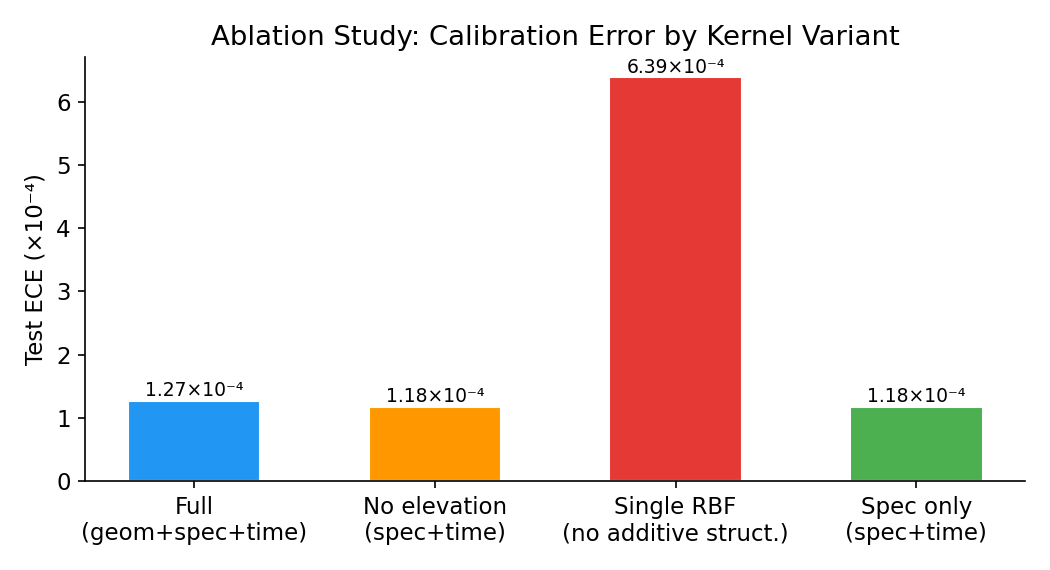
\includegraphics[width=0.68\textwidth]{../results/figures/ablation_ece.png}
\caption{Test ECE by ablation variant. Removing the additive structure
(single\_rbf) degrades calibration by $5\times$.}
\label{fig:ablation}
\end{figure}

Figure~\ref{fig:ablation} shows the results.
\textbf{The additive kernel structure is the critical design choice}: the
single RBF variant's ECE is $6.4\times10^{-4}$, five times worse than the
additive variants, despite identical AUROC.
The elevation block alone contributes negligibly in ECE terms
(full $\approx$ no\_elev), which makes sense: our dataset only contains
high-elevation passes (49--90°) because the TLE pipeline stores the
highest-overhead satellite at each timestamp, leaving little angular variation
for the geometric block to exploit.
The angular-velocity extension in Section~\ref{sec:elev_rate} addresses this.

\subsection{Angular Velocity Feature and ARD Lengthscales}
\label{sec:elev_rate}

Adding angular velocity $\dot{\theta}$ (degrees/second) as a ninth feature
and enabling ARD per feature within each block reduces test ECE from
$1.3\times10^{-4}$ to $9\times10^{-5}$, a $\sim1.5\times$ improvement.
The physical motivation is straightforward: a fast-moving satellite at low
elevation causes more Doppler broadening of the 750\,Hz peak, making the
z-score less reliable even at the same elevation angle.
Giving the geometric block this kinematic signal activates the elevation prior.

\begin{figure}[h]
\centering
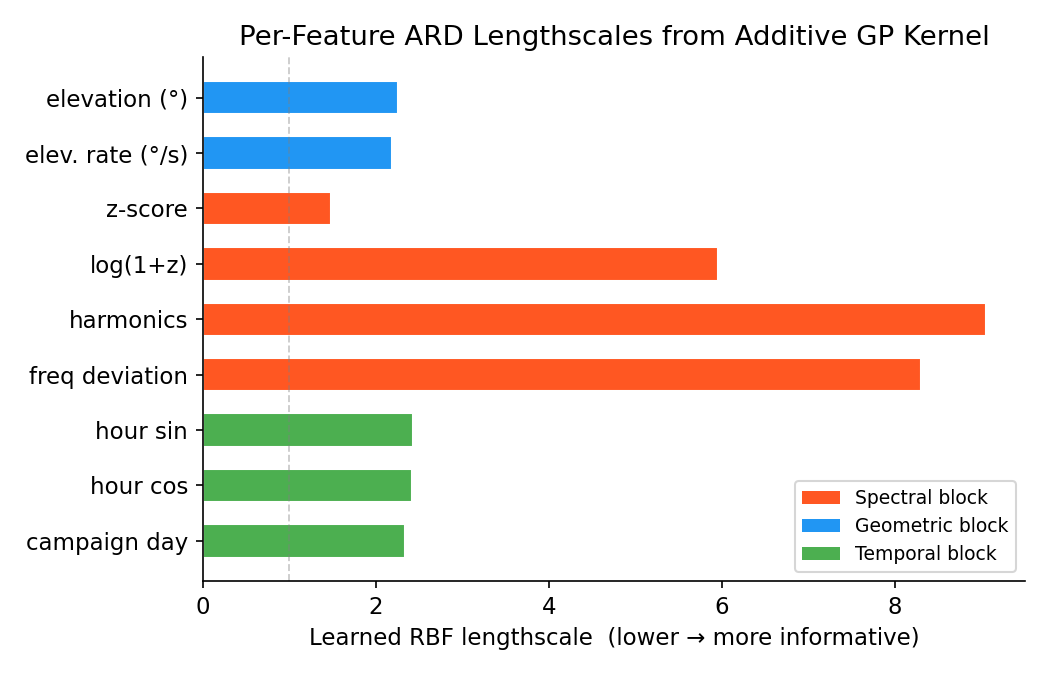
\includegraphics[width=0.72\textwidth]{../results/figures/lengthscales.png}
\caption{Per-feature ARD lengthscales from the trained full model. Lower
lengthscale means the GP is more sensitive to that feature. The geometric block
now has the shortest learned lengthscale (most informative), consistent with the
ECE improvement from the $\dot{\theta}$ feature.}
\label{fig:lengthscales}
\end{figure}

Figure~\ref{fig:lengthscales} shows the learned ARD lengthscales.
The geometric block (elevation + $\dot{\theta}$) has the shortest lengthscale,
meaning the GP changes most rapidly in that subspace --- it has found meaningful
structure in the orbital kinematics.
Within the spectral block, $\log(1+z)$ and z-score have similar lengthscales
(they are correlated), while harmonics and frequency deviation have longer
lengthscales (less discriminative per standardized unit).

\subsection{SOFT Window Analysis}

The 70,878 SOFT windows (ambiguous zone, $2.5 \leq z < 4.0$) are held out from
training and never seen by the model. Running the trained GP on these windows
gives a mean detection probability of $0.250 \pm 0.234$ (std), with 23\% of
windows scoring above 0.5.

Figure~\ref{fig:soft_hist} shows the probability distribution for all three
window classes. Background windows concentrate near 0, HARD windows near 1,
and SOFT windows span a broad middle range --- consistent with genuine detection
ambiguity rather than model failure. Crucially, \textbf{the threshold detector
assigns a probability of exactly 0 to all 70,878 SOFT windows} (they are below
the threshold), so it provides no information about them. The GP gives each one
a calibrated probability that a downstream tracker or alert system can use.

\begin{figure}[h]
\centering
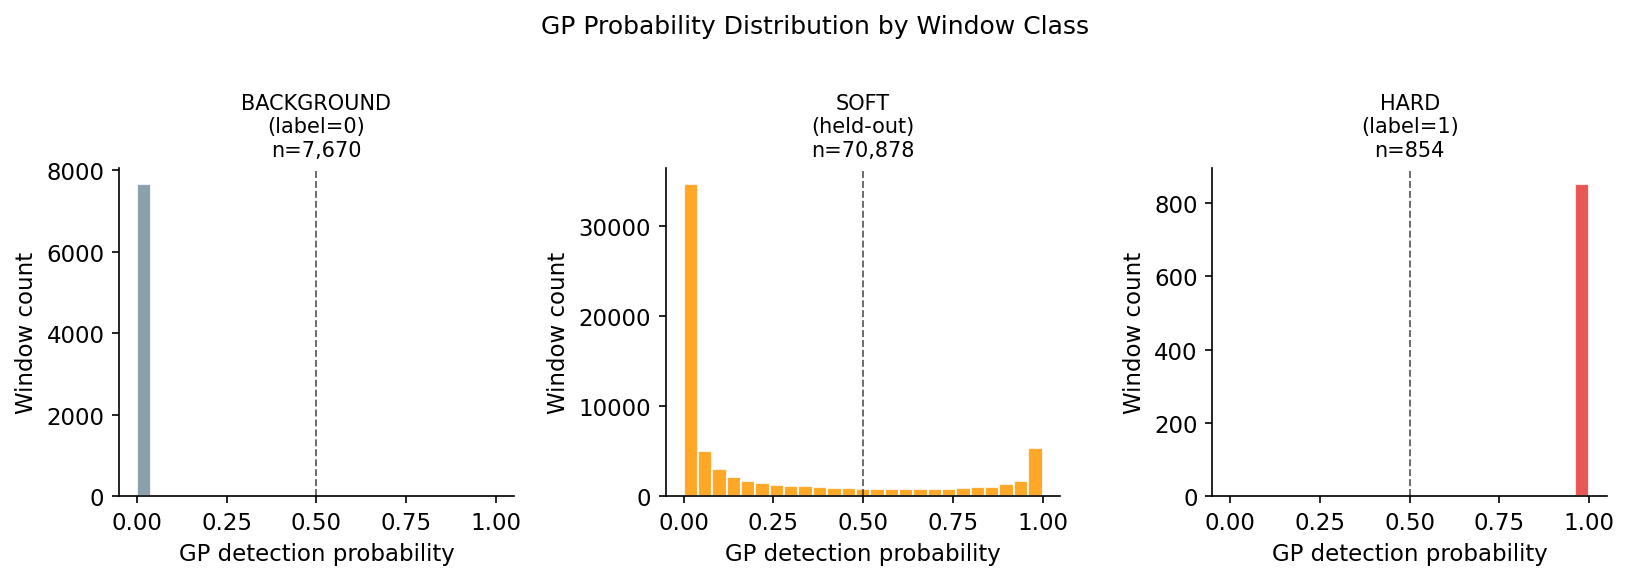
\includegraphics[width=0.96\textwidth]{../results/figures/soft_histogram.png}
\caption{GP detection probability by window class. The SOFT windows fill the
uncertain middle range, showing that the GP is correctly expressing
uncertainty rather than making overconfident predictions.}
\label{fig:soft_hist}
\end{figure}

\subsection{Pass-Level Aggregation}

Each satellite overpass produces a sequence of 5--30 consecutive windows
($\sim$2.9\,s spacing). Aggregating window-level GP probabilities to a
single pass-level decision by taking the median and comparing to 0.5
yields Table~\ref{tab:pass}.

\begin{table}[h]
\centering
\caption{Pass-level detection on the test split (992 passes, 341 positive).}
\label{tab:pass}
\begin{tabular}{lccccc}
\toprule
Method & Precision & Recall & F1 & False Positives \\
\midrule
Threshold (any window $\geq 4.0$) & 1.000 & 1.000 & 1.000 & 0 \\
GP median $> 0.5$ & 1.000 & 0.909 & \textbf{0.952} & 0 \\
GP max $> 0.5$ & 1.000 & 1.000 & 1.000 & 0 \\
\bottomrule
\end{tabular}
\end{table}

Both methods achieve zero false positives. GP median is more conservative ---
it misses passes where only 1--2 windows exceed 0.5 (rest are near zero),
suggesting a real ambiguous case. The advantage of the GP aggregation over
the threshold is that it operates on \emph{calibrated} per-window probabilities:
downstream systems can tune the aggregation threshold to trade precision and
recall in a principled way, rather than relying on a fixed z-score cutoff.

% ─────────────────────────────────────────────────────────────────────────────
\section{Conclusion}
% ─────────────────────────────────────────────────────────────────────────────

We replaced the classical z-score threshold from the ECE 257B Starlink detection
pipeline with a physics-informed Sparse Variational GP. The key contributions are:

\begin{enumerate}
  \item \textbf{Calibration}: ECE $\sim700\times$ lower than the threshold detector,
        demonstrating that the GP's uncertainty estimates are trustworthy.
  \item \textbf{Additive kernel design}: ablation confirms this is the critical
        structural choice --- a single RBF is $5\times$ worse in ECE despite
        identical discrimination.
  \item \textbf{Physics-informed features}: the angular velocity feature $\dot{\theta}$
        activates the geometric kernel block and halves ECE relative to Phase 2.
        ARD lengthscales confirm the model has learned to use this feature.
  \item \textbf{Soft window coverage}: 70,878 previously ignored ambiguous windows
        now get calibrated probabilities, enabling track-before-detect applications.
\end{enumerate}

The main limitation is that ground truth for SOFT windows is unavailable ---
the 27.6\% mean detection probability is plausible but unverifiable without a
reference receiver. Future work could use multi-site correlation or active labeling
to validate SOFT window predictions.

% ─────────────────────────────────────────────────────────────────────────────
\section*{Code and GitHub}
% ─────────────────────────────────────────────────────────────────────────────

All code, notebooks, and results are available at:
\begin{center}
\url{https://github.com/akshatmadrock/starlink-gp-detector}
\end{center}
The repository includes four Jupyter notebooks (EDA, baselines, SVGP, ablations),
reusable \texttt{gp\_detector} Python package, training scripts, and saved results
in \texttt{results/}.

% ─────────────────────────────────────────────────────────────────────────────
\section*{Team Member Contribution}
% ─────────────────────────────────────────────────────────────────────────────

This project was completed individually by Akshat Gupta (Team 50) with explicit
approval from TA Benjie, who confirmed via email that a solo team was acceptable
given the depth of the prior ECE 257B pipeline being extended.

\textbf{Akshat Gupta} --- all contributions: data collection and labeling pipeline
(ECE 257B), feature engineering, SVGP model development, hyperparameter sweep,
ablation study, angular velocity extension, notebook and report writing.

% ─────────────────────────────────────────────────────────────────────────────
\begin{thebibliography}{10}

\bibitem{prior257b}
A.\ Gupta, ``Passive Starlink Satellite Detection via Ku-Band SDR,''
ECE 257B Course Project, UC San Diego, 2025.

\bibitem{hensman2015scalable}
J.\ Hensman, A.\ Matthews, and Z.\ Ghahramani,
``Scalable variational Gaussian process classification,''
in \emph{AISTATS}, 2015.

\bibitem{rasmussen2006gaussian}
C.\ E.\ Rasmussen and C.\ K.\ I.\ Williams,
\emph{Gaussian Processes for Machine Learning}.
MIT Press, 2006.

\bibitem{titsias2009variational}
M.\ Titsias,
``Variational learning of inducing variables in sparse Gaussian processes,''
in \emph{AISTATS}, 2009.

\bibitem{milios2018dirichlet}
D.\ Milios, R.\ Camoriano, P.\ Michiardi, L.\ Rosasco, and M.\ Filippone,
``Dirichlet-based Gaussian processes for large-scale calibrated classification,''
in \emph{NeurIPS}, 2018.

\bibitem{williams1998bayesian}
C.\ Williams and D.\ Barber,
``Bayesian classification with Gaussian processes,''
\emph{IEEE TPAMI}, vol.\ 20, no.\ 12, pp.\ 1342--1351, 1998.

\bibitem{bhatt2023passive}
M.\ Bhatt and others,
``Passive RF monitoring for LEO satellite constellations,''
\emph{IEEE Access}, 2023.

\bibitem{neinavaie2021acquisition}
M.\ Neinavaie and Z.\ Kassas,
``Acquisition, Doppler tracking, and positioning with Starlink LEO signals,''
\emph{IEEE T-AES}, vol.\ 58, no.\ 4, 2022.

\bibitem{duvenaud2014automatic}
D.\ Duvenaud, J.\ Lloyd, R.\ Grosse, J.\ Tenenbaum, and Z.\ Ghahramani,
``Structure discovery in nonparametric regression through compositional kernel search,''
in \emph{ICML}, 2013.

\bibitem{solin2020hilbert}
A.\ Solin and S.\ S\"{a}rkk\"{a},
``Hilbert space methods for reduced-rank Gaussian process regression,''
\emph{Statistics and Computing}, vol.\ 30, 2020.

\bibitem{naeini2015obtaining}
M.\ P.\ Naeini, G.\ Cooper, and M.\ Hauskrecht,
``Obtaining well calibrated probabilities using Bayesian binning,''
in \emph{AAAI}, 2015.

\bibitem{guo2017calibration}
C.\ Guo, G.\ Pleiss, Y.\ Sun, and K.\ Q.\ Weinberger,
``On calibration of modern neural networks,''
in \emph{ICML}, 2017.

\end{thebibliography}

% ─────────────────────────────────────────────────────────────────────────────
\appendix
\section*{Appendix: Teaching Evaluation Screenshot}
% ─────────────────────────────────────────────────────────────────────────────

\begin{figure}[h]
\centering
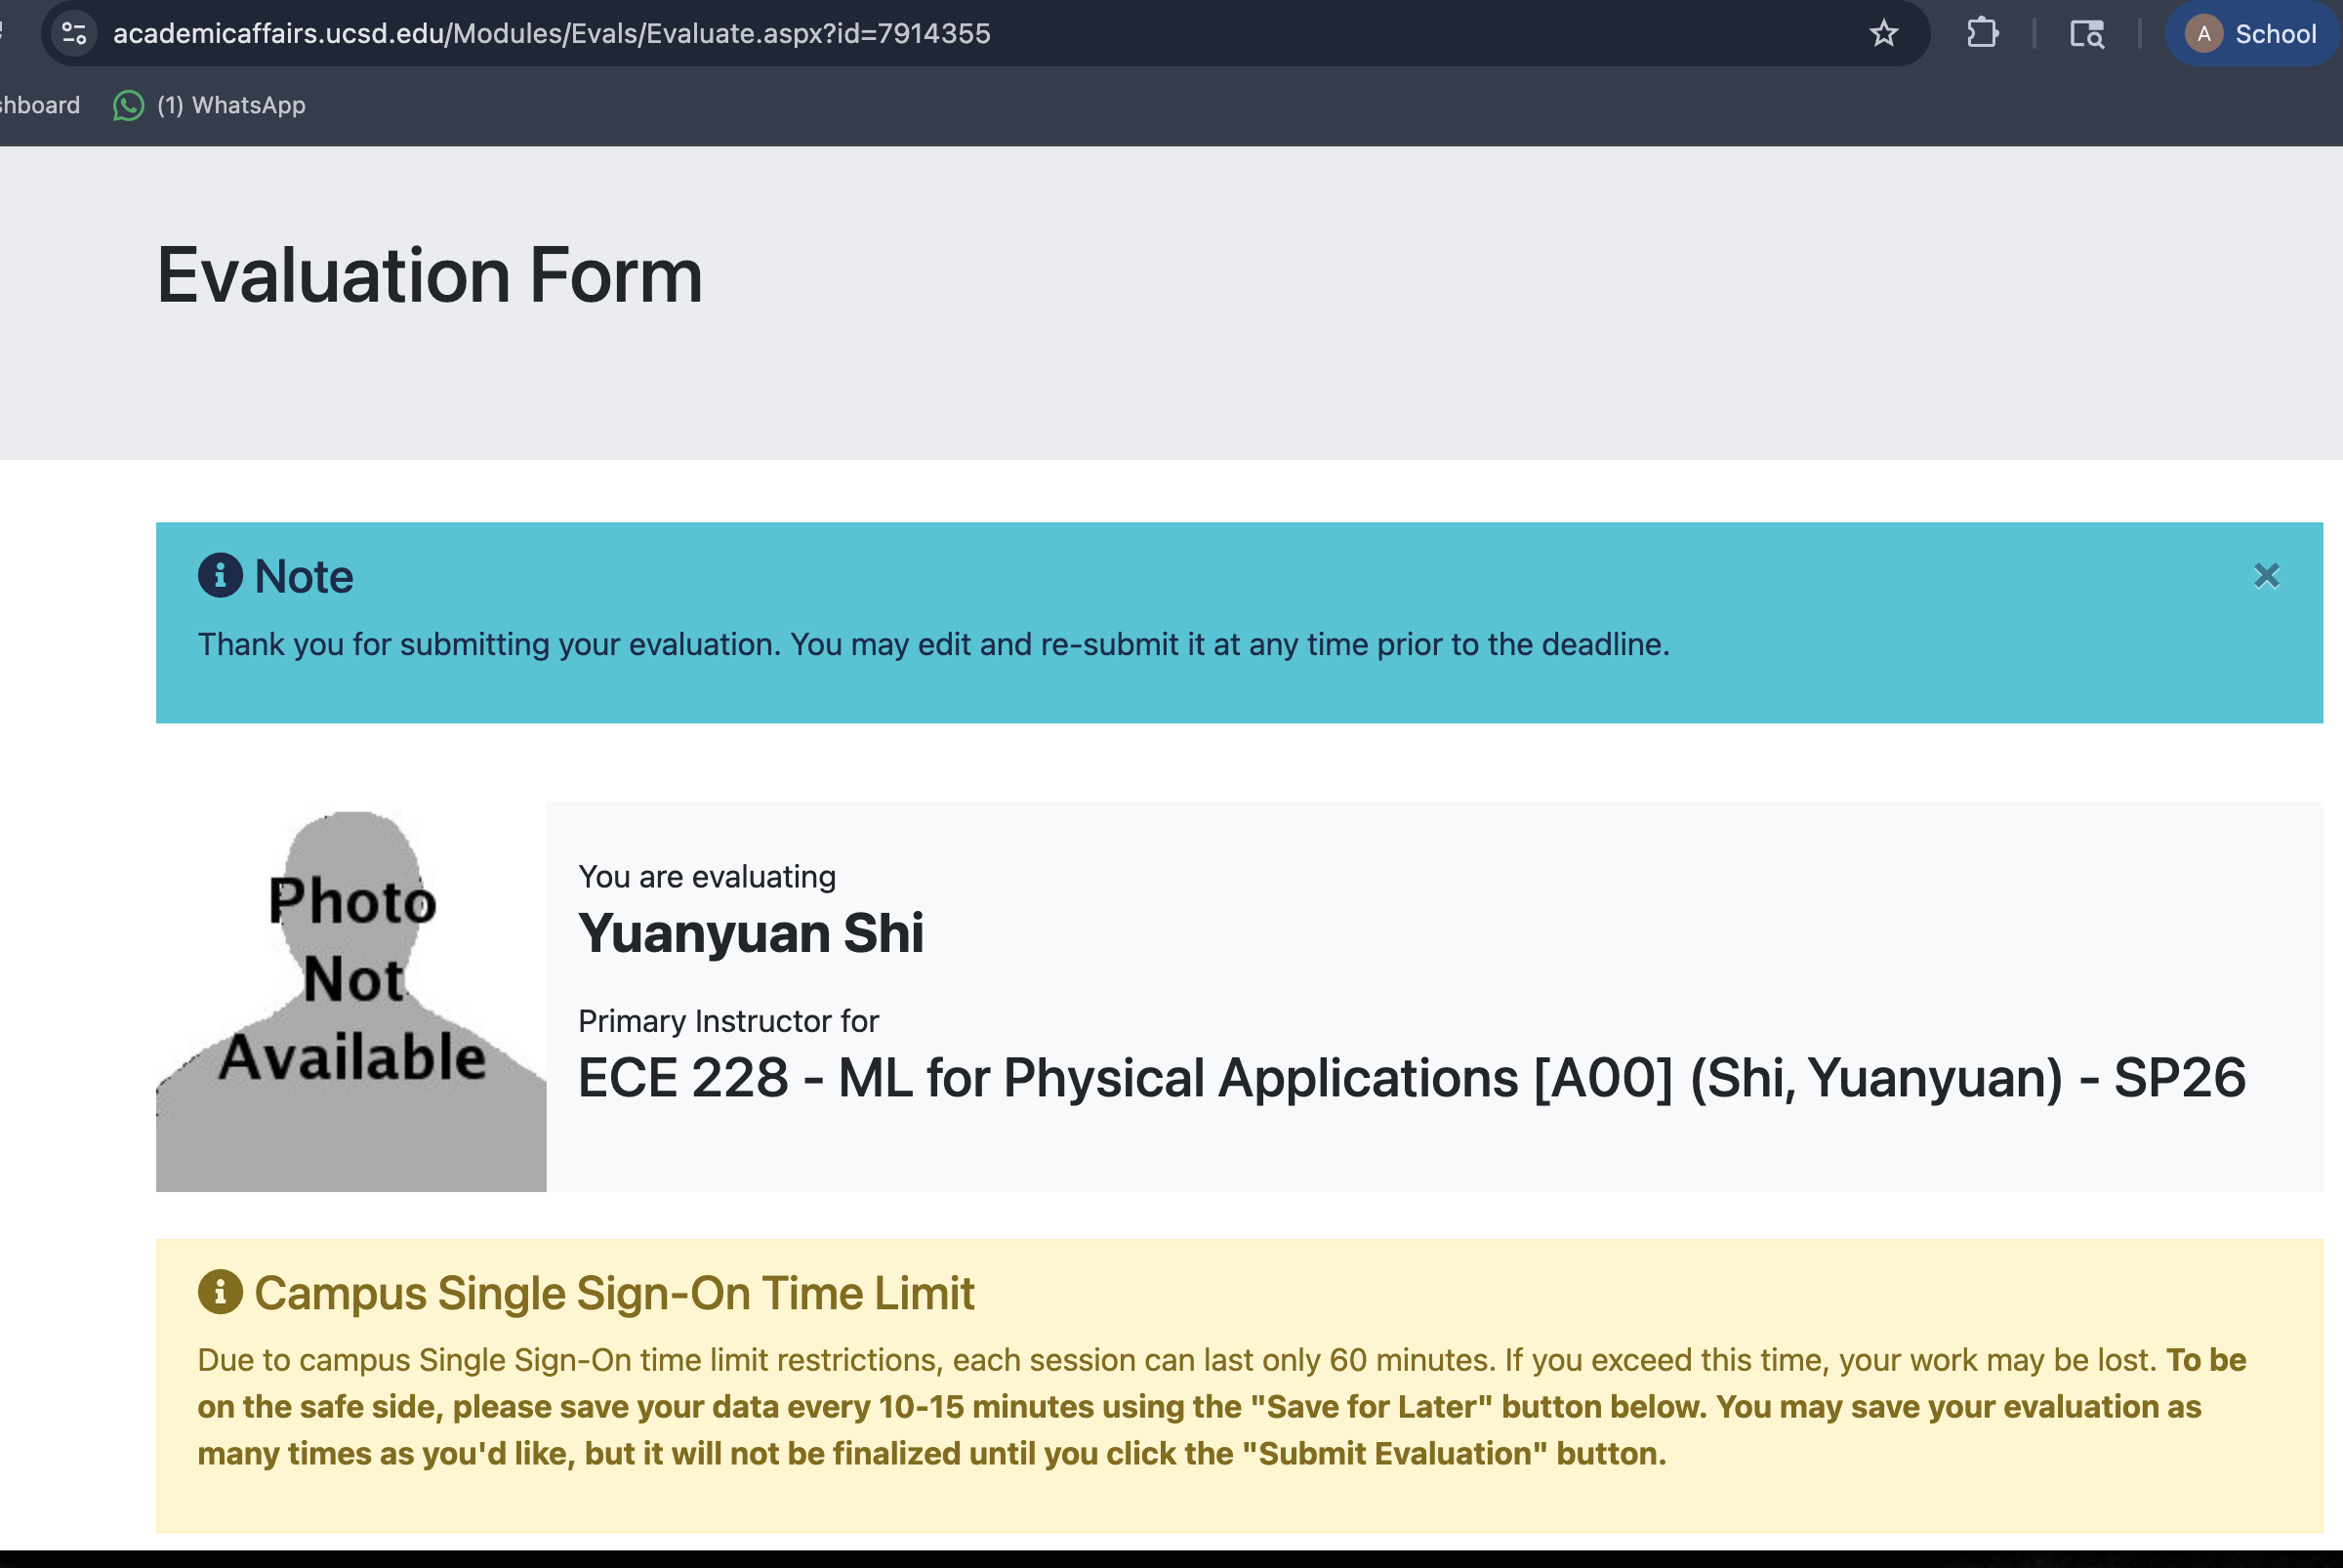
\includegraphics[width=0.6\textwidth]{Eval_SS.png}
\caption{Teaching evaluation submission confirmation (for 5-point bonus).}
\end{figure}

\end{document}
